\subsection{MEX 3-1: CNL direct shear test data (TUBAF)}\label{DataManMex3-1CNL}\index{Constant Normal Load (CNL) experiment}

Participating institutions of MEX 3-1 (see section \ref{sec:mex07}): TUBAF

\begin{table}[ht!]
\caption{MEX 3-1: Data overview}
\label{tab:dms-mex31-overview}
\small
\begin{tabular}{l|l|l|l|L{4.7cm}|l}
\hline
\rowcolor{cyan}
Type & Spec. & Owner & Access     & Comment                 & Stat \\ 
\hline 
EXP  & LAB   & TUBAF & Limited    & Available, UFZ-DMP      & \cellcolor{green} \\
\hline \hline
MOD  & FFS   & TUBAF & Open source & Available via GitHub   & \cellcolor{green} \\
     &       &       & Free       & I/O available           & \cellcolor{green} \\
\hline
\end{tabular}
\end{table}
\normalsize

Link to the data set at UFZ data portal (DMP):\\ \url{www.ufz.de/record/dmp/archive/7925/}

The CNL data set contains four text files. One text file with the rock properties of the used granite (see Tab. \ref{table:MEX7_rockParam}). Two files with the scan data of the two surfaces. One point cloud can be seen in Fig. \ref{fig:DataCNLGranitePointCloud}. The last file contains the laboratory data. In Fig. \ref{fig:DataCNLGraniteLab} the results for the four shear stress levels can be seen.

\begin{figure}[!ht]
\begin{center}
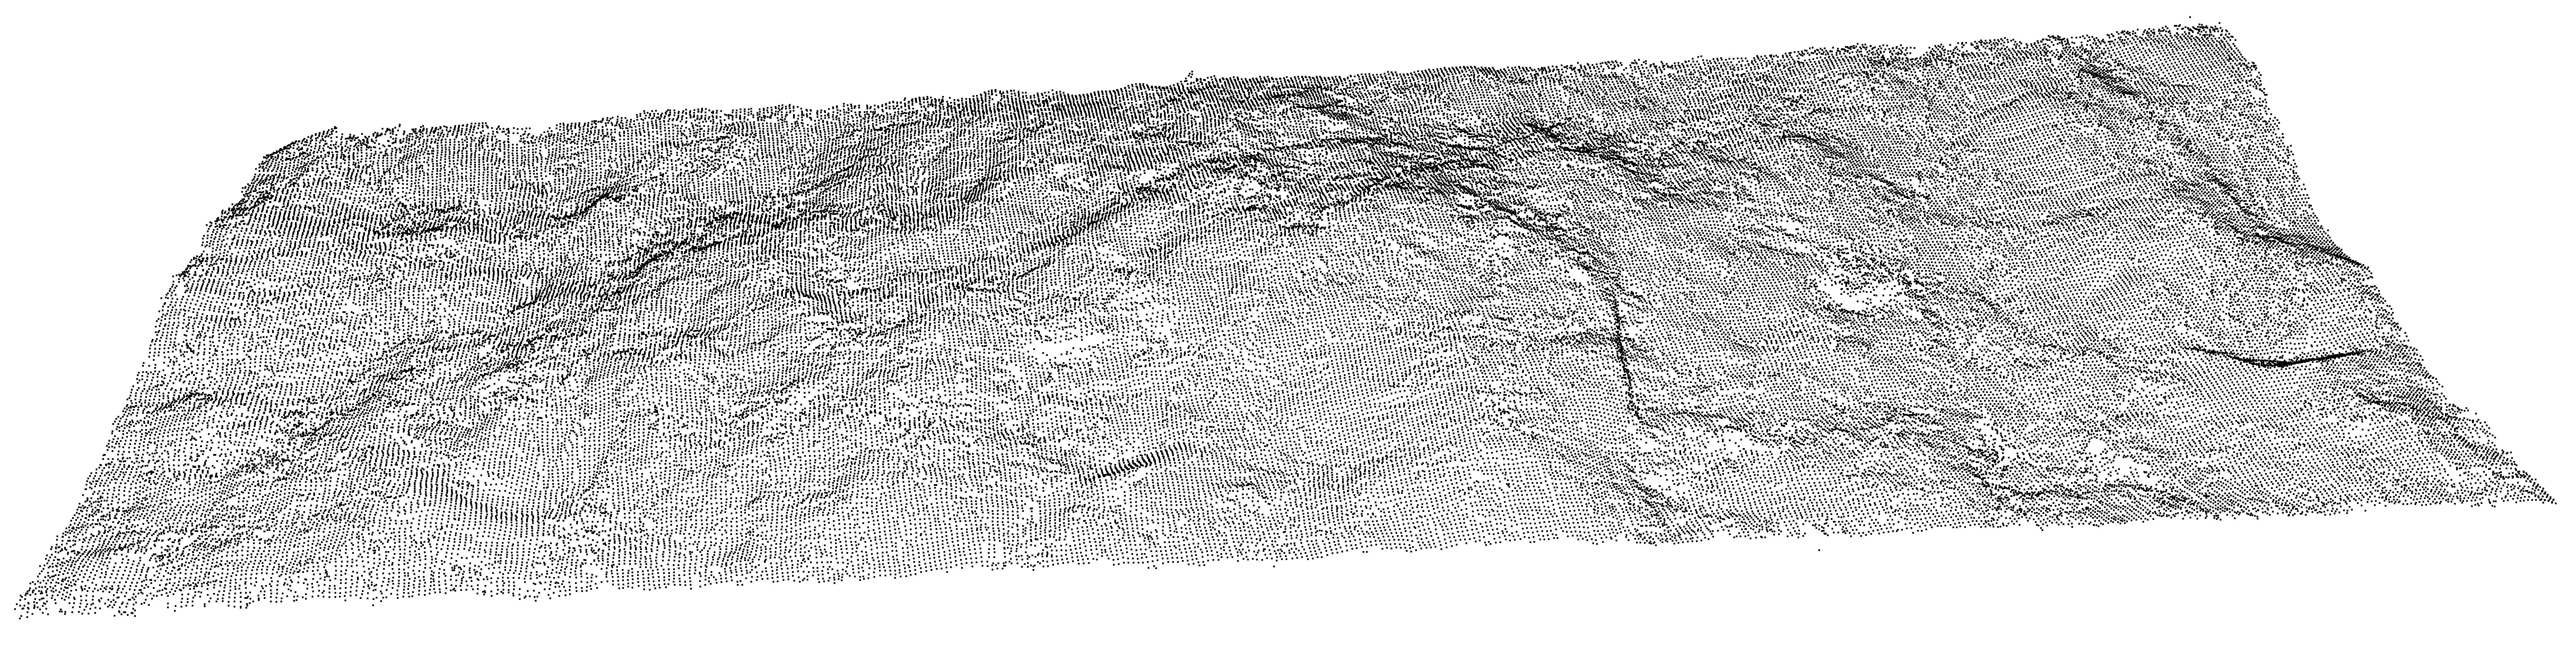
\includegraphics[width=0.85\textwidth]{./figures/MEX7_Point_cloud.png}
\end{center}
\caption{Point cloud representing the surface of a granite sample from Saxony. The size is 65 mm by 170 mm and the cloud contains approx. 98000 points.}
\label{fig:DataCNLGranitePointCloud}
\end{figure}

\begin{figure}[!ht]
\begin{tabular}{cc}
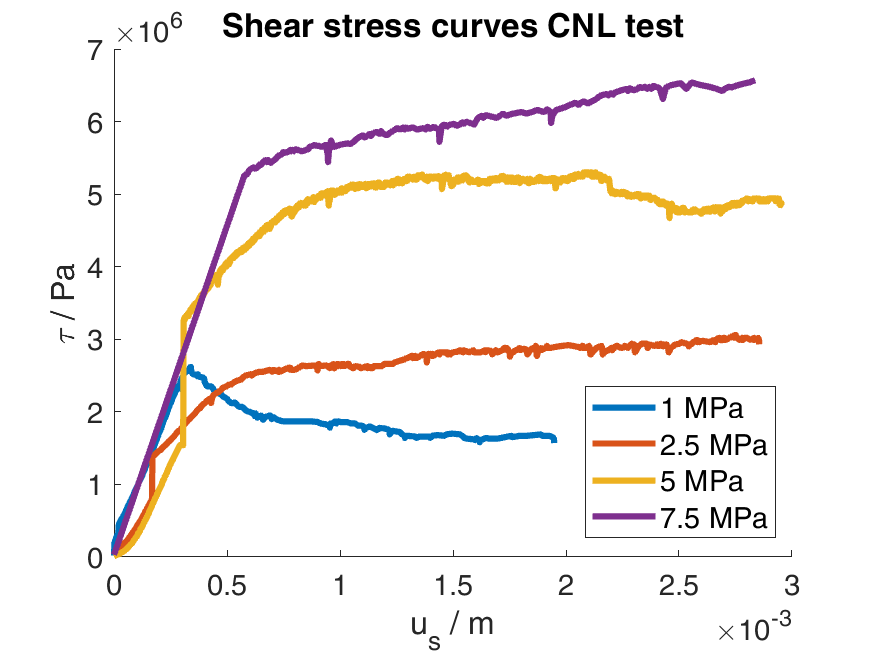
\includegraphics[width=0.48\textwidth]{./figures/CNLShearCurvesAll.png}     
& 
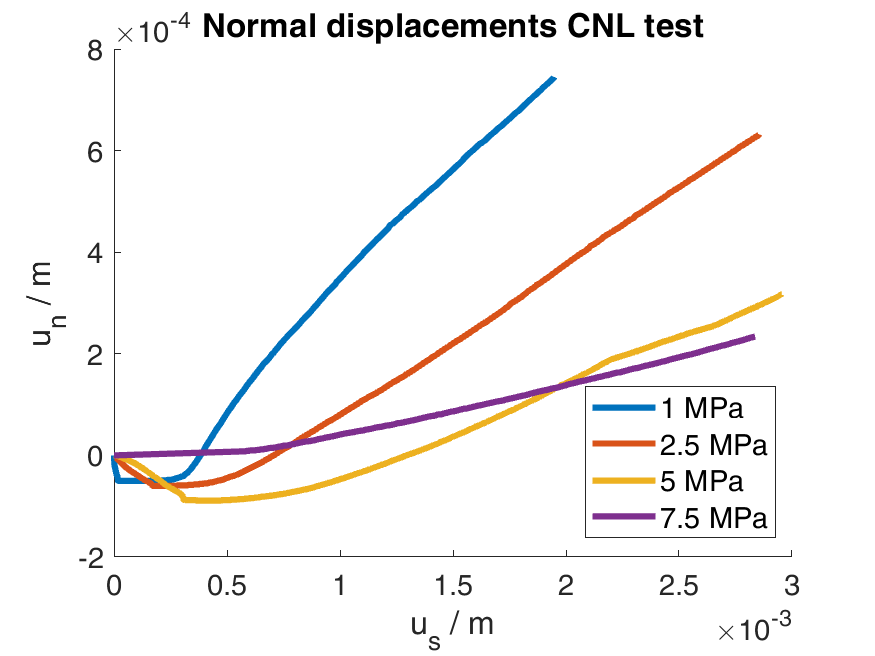
\includegraphics[width=0.48\textwidth]{./figures/CNLDilatationAll.png} 
\end{tabular}
\caption{CNL test results}
\label{fig:DataCNLGraniteLab}
\end{figure}

\clearpage
%---------------------------------------------------------
\subsubsection*{Meta Data Overview (according to Dublin Core)}
%---------------------------------------------------------

\begin{table}[!ht]
\caption{MEX 3-1 (TUBAF)}
\label{tab:dms-mex3-1}
\small
\begin{tabular}{R{3cm}|L{7cm}}
\hline
%\rowcolor{Cyan}
%
Data label & GeomInt | TUBAF | Data Set CNL \\
URL & http://www.ufz.de/record/dmp/archive/7925 \\
Subject  & Crystalline rock, direct shear test \\
Type of data  & collection of various data \\
Data quality  & quality assured data \\
Status of data  & processed data \\
Data format  & txt, jpg, png \\
Creators  & TU Freiberg, Institut für Geotechnik, Gustav-Zeuner-Str. 1, 09599 Freiberg \\
Source/Origin  & Rock mechanical laboratory \\
Publisher  & TU Freiberg, Institut für Geotechnik, Gustav-Zeuner-Str. 1, 09599 Freiberg \\
Rights holders  & TU Freiberg, Institut für Geotechnik, Gustav-Zeuner-Str. 1, 09599 Freiberg \\
Contributors  & TU Freiberg, Institut für Geotechnik, Thomas Fr\"uhwirt and Daniel P\"otschke \\
Time/period of creation  & 2018 - 2019 \\
Language of the content & English \\
Update policy  & Stored data will not be extended \\
Access permissions  & Limited access \\
%
\hline
\end{tabular}
\end{table}